\section{Progettazione di una base di dati}
\subsection{Anomalie}
Si immagini di dover progettare una base di dati relazionale contenente i dati degli 
studenti e dei corsi di un'Università. La soluzione più immediata è di creare un'unica
relazione
\begin{center}
  $Universit\grave{a}(Matr, Nome, Citt\grave{a}, Prov, C\#, Titolo, Docente, C\_laurea,
  Data, Voto)$ 
\end{center}

in cui una tupla $(m, n, c, p, C, t, D, l, d, v)$ rappresenta il fatto che uno studente
con matricola $m$ e nome $n$, residente nella città $c$ che si trova in provincia di $p$,
ha sostenuto l'esame del corso, con codice $C$ e titolo $t$, tenuto dal docente $D$, del 
corso di laurea $l$ in data $d$ riportando il voto $v$.\\\\
Adottando questa soluzione si avrebbero un certo numero di inconvenienti che vanno sotto 
il nome di \textbf{anomalia}. Un anomalia è essenzialmente un comportamento \emph{inaspettato
e indesiderato} da parte della base di dati, generato in risposta ad un'operazione. Le anomalie 
più comuni (spiegate relativamente all'esempio) sono:
\begin{itemize}
 \item \textbf{anomalie di inserimento}: non si possono inserire i dati di uno studente 
 se non ha sostenuto almeno un esame;
 \item \textbf{anomalie di cancellazione}: se si cancellano i dati di un corso (perché il
 corso è stato disattivato) e c'è uno studente che ha sostenuto solo l'esame relativo a 
 quel corso, perdo le informazioni sullo studente;
 \item \textbf{anomalie di aggiornamento}: se devo modificare il docente di un corso devo 
 farlo per ogni tupla in cui compare il corso;
 \item \textbf{ridondanza} dei dati: le informazioni anagrafiche di uno studente sono
  ripetute per ogni esame sostenuto dallo studente.
\end{itemize}
Queste anomalie sono dovute al fatto che si sono rappresentati in un'unica relazione più 
\emph{concetti}: il concetto ``Studente'', ``Corso'' ed ``Esame''. Rappresentando i tre 
concetti in tre relazioni distinte
\begin{center}
  $Studente(Matr, Nome, Citt\grave{a}, Prov)$\\
  $Corso(C\#, Titolo, Docente, C\_laurea)$\\
  $Esame(Matr, C\#, Data, Voto)$
\end{center}

tali anomalie vengono eliminate. Tuttavia è possibile riscontrare il permanere di simili 
anomalie concernenti le città: per eliminare queste ultime anomalie che hanno la stessa 
origine di quelle viste precedentemente, posso utilizzare lo \emph{schema} seguente:
\begin{center}
  $Studente(Matr,Nome,Citt\grave{a})$\\
  $Comune(Citt\grave{a},Prov)$\\
  $Corso(C\#,Titolo,Docente, C\_laurea)$\\
  $Esame(Matr, C\#, Data,Voto)$
\end{center}

\subsection{La Terza Forma Normale}
Si è constatato che ci sono schemi migliori di altri. Esistono dunque \emph{regole 
e proprietà formali} che ci permettono di costruire un \emph{buono} schema?
Se si analizzano le anomalie nella relazione $Universit\grave{a}$ si nota che sono 
legate al fatto che
\begin{itemize}
 \item $Voto$ e $Data$ sono \emph{determinati univocamente} da $Matr$ e $C\#$;
 \item  i dati di uno studente sono \emph{determinati univocamente} da $Matr$;
 \item i dati di un corso sono \emph{determinati univocamente} da $C\#$.
\end{itemize}
Il concetto di ``determina univocamente'' è colto dal concetto formale di \emph{dipendenza funzionale}.
\begin{defn}
  Dato uno schema di relazione $R$, una \textbf{dipendenza funzionale} su $R$ 
  è una coppia ordinata di sottoinsiemi non vuoti $X$, $Y$ $\in R$ e viene denotata 
  come $X \rightarrow Y$.
\end{defn}

\begin{prop}
Un'istanza $r$ di $R$ \emph{soddisfa} la dipendenza funzionale $X \rightarrow Y$
se per ogni coppia di tuple $t_1$, $t_2$ $\in r$ si ha che se $t_1[X] = t_2[X] 
\Rightarrow t_1[Y] = t_2[Y]$. 
\end{prop}
In simboli:
\begin{center}
\begin{math}
(\ \forall (t_1, t_2) \in r\ t.c.\ t_1[X] = t_2[X] \Rightarrow t_1[Y] = t_2[Y]) 
\Rightarrow (r
\end{math}
soddisfa $X\rightarrow Y$).
\end{center}
Sia $F$ un insieme di dipendenze funzionali su $R$ ed $r$ un'istanza di $R$. Se $r$ 
soddisfa tutte le dipendenze in $F$, diciamo che $r$ è un'istanza \emph{legale} di $R$. 
\begin{defn}
La \textbf{chiusura di F}, denotata con $F^+$, è l'insieme di dipendenze funzionali che 
sono soddisfatte da ogni istanza legale di $R$. 
\end{defn}

Banalmente si ha che $F$ $\subseteq$ $F^+$.\\
\label{defn_4_3}
\begin{defn}
 Dato uno schema di relazione $R$, un insieme di dipendenze funzionali $F$ su $R$ e un
sottoinsieme $K$ di $R$, diciamo che $K$ è una \textbf{chiave} per $R$ se:
\begin{itemize}
 \item $K \rightarrow R \in F^+$
 \item $\forall K'\subset K,\ K'\rightarrow R \notin F^+$.
\end{itemize}
\end{defn}
In pratica una chiave è il minimo sottoinsieme di $R$ che determina univocamente il 
valore dei restanti attributi di $R$ (banalmente la chiave determina se stessa e i 
suoi sottoinsiemi) tale che, se prendessimo un suo sottoinsieme, esso non sarebbe 
chiave.\\
In futuro denoteremo con $A_1, A_2, \ldots, A_n$ un insieme di attributi, con $X$ 
e $Y$ sottoinsiemi di $R$, con $XY$ l'insieme $X$ $\cup$ $Y$.

\begin{exmp}
 Considerando il precendente schema $Universit\grave{a}$, possiamo osservare che un'istanza 
 di \emph{Università} per rispecchiare la realtà di interesse deve soddisfare le seguenti 
 dipendenze funzionali:
 \begin{itemize}
  \item $Matr,\ C\# \rightarrow Nome,\ Citt\grave{a},\ Prov,\ Titolo,\ Docente,\ C\_laurea,
  \ Data,\ Voto$;
  \item $C\# \rightarrow Titolo,\ Docente,\ C\_laurea$
  \item $Matr \rightarrow Nome,\ Citt\grave{a},\ Prov$
  \item $Citt\grave{a} \rightarrow Prov$
 \end{itemize}
 Quindi $\{Matr, C\#\}$ costituisce una \emph{chiave} per Università.
\end{exmp}

Ci sono attributi che \textbf{dipendono parzialmente} dalla chiave. Nell'\textsc{Esempio 4.1} 
\{$Titolo$, $Docente$, $C\_laurea$\} dipendono funzionalmente da $C\#$; altri attributi
invece \textbf{dipendono transitivamente} dalla chiave, ad esempio $Prov$ dipende
funzionalmente da $Matr$ in quanto $Matr \rightarrow Citt\grave{a} \rightarrow Prov$.\\
Prendendo lo schema finale, vediamo che in nessuno schema di relazione ci sono attributi
che dipendono parzialmente né transitivamente dalla chiave. 
\begin{prop}
Uno schema di relazione in cui non ci sono sono attributi che dipendono parzialmente né 
transitivamente dalla chiave è detto in \textbf{Terza Forma Normale} (3NF). 
\end{prop}
Formalizziamo i concetti appena introdotti:
\begin{defn}
 Dati uno schema di relazione $R$ e un insieme di dipendenze funzionali $F$ su $R$
diciamo che:
\begin{itemize}
 \item un attributo $A$ $\in$ $R$ è \textbf{primo} se appartiene ad una chiave di $R$;
 \item un sottoinsieme $X$ $\subset$ $R$ è una \textbf{superchiave} se contiene una 
 chiave di $R$.
\end{itemize}
\end{defn}
Nell'\textsc{Esempio 4.1}, considerando la relazione \emph{Università}, $Matr$ è primo mentre
 \{$Matr$, $C\#$, $Nome$\} è una superchiave.
\begin{defn}
Siano $R$ uno schema di relazione ed $F$ un insieme di dipendenze funzionali su $R$.
\begin{itemize}
 \item $X\rightarrow A$ $\in F^+$ è una \textbf{dipendenza parziale} su $R$ se $A$ non 
 è primo e $X$ è contenuto propriamente in una chiave di R.
 \item $X\rightarrow A$ $\in F^+$ è una \textbf{dipendenza transitiva} su $R$ se $A$ 
 non è primo e $\forall K \subset R$, dove $K$ è chiave, si ha che $X$ non è contenuto propriamente 
 in $K$ e $K-X \neq \emptyset$.
\end{itemize}
\end{defn}
\begin{defn}
Siano $R$ uno schema di relazione ed $F$ un insieme di dipendenze funzionali su $R$. 
$R$ è in 3NF se, $\forall (X\rightarrow A) \in F^+$ t.c. $A\notin X$, si ha che $A$ è
primo oppure $X$ è una superchiave.
\end{defn}
\begin{theo}
Siano $R$ uno schema di relazione e $F$ un insieme di dipendenze funzionali su $R$. Uno
schema $R$ è in 3NF se e solo se non esistono né dipendenze parziali né dipendenze 
transitive in $R$.
\end{theo}
\textbf{Dimostrazione.} La parte \emph{solo se} è banale dopo aver visto la parte \emph{se}.\\
\emph{Parte se}. Supponiamo per assurdo che $R$ non sia in 3NF nonostante non ci siano
dipendenze parziali o transitive; in tal caso esiste una dipendenza funzionale $X\rightarrow A$
$\in F^+$ t.c. $A$ non è primo e $X$ non è una superchiave. Poiché $X$ non è una
superchiave due casi (mutuamente esclusivi) sono possibili:
\begin{itemize}
 \item o per ogni chiave $K$ di $R$, $X$ non è contenuto propriamente in $K$ e $K-X \neq 
 \emptyset$; in tal caso $X\rightarrow A$ è una dipendenza transitiva su $R$ (contraddizione)
 \item oppure esiste una chiave $K$ di $R$ t.c. $X \subset K$; in tal caso $X\rightarrow A$ 
 è una dipendenza parziale su $R$ (contraddizione).\hfill $\Box$
\end{itemize}
Un obbiettivo da tenere presente quando si progetta una base di dati è quello di produrre 
uno schema in cui ogni relazione sia in 3NF. Nella fase di progettazione concettuale si 
individuano i concetti che devono essere rappresentati nella base di dati. Se questo lavoro 
di individuazione è fatto accuratamente lo schema relazionale che può essere derivato in modo
automatico con opportune regole, è in 3NF. Se tuttavia dopo tale processo ci trovassimo a 
produrre uno schema che non è in 3NF dovremmo procedere ad una fase di decomposizione.

\subsection{Decomposizione di schemi di relazione}
Uno schema che non è in 3NF può essere decomposto in più modi in un insieme di schemi in 3NF.\\
 Sia $R = ABC$ con l'insieme di dipendenze funzionali $F = \{A\rightarrow B, B\rightarrow C\}$.
$R$ non è in 3NF per la presenza in $F^+$ della dipendenza transitiva $B\rightarrow C$, ma può 
essere decomposto in:
\begin{center}
  $R_1 = AB$ con $F_1=\{A\rightarrow B\}$\\
  $R_2 = BC$ con $F_2=\{B\rightarrow C\}$\\
  oppure\\
  $R_1 = AB$ con $F_1=\{A\rightarrow B\}$\\
  $R_2 = AC$ con $F_2=\{A\rightarrow C\}$\\
\end{center}
Entrambi gli schemi sono in 3NF, tuttavia la seconda soluzione non è soddisfacente. Infatti,
si consideri l'istanza della \emph{base di dati} costituita dalle due istanze legali di $R_1$ e $R_2$:

    \begin{multicols}{2}   
    \begin{flushright}
    \begin{tabular}{l|l}
     A & B \\
     \hline
     $a_1$ & $b_1$\\
     $a_2$ & $b_1$
    \end{tabular}
    \end{flushright}

    \begin{flushleft}
    \begin{tabular}{l|l}
     A & C \\
     \hline
     $a_1$ & $c_1$\\
     $a_2$ & $c_2$
    \end{tabular}
    \end{flushleft}
    \end{multicols}  
 
  L'istanza di R che si può ricostruire da questa tramite \emph{join naturale} è\\
    \begin{center}
    \begin{tabular}{l|l|l}
     A & B & C \\
     \hline
     $a_1$ &$b_1$ & $c_1$\\
     $a_2$ &$b_1$ & $c_2$
    \end{tabular}
    \end{center}
    
    non è un'istanza legale di $R$, in quanto non soddisfa la dipendenza funzionale
    $B\rightarrow C$.
 \label{esempio_4_2}
 \begin{exmp}
  Si consideri la relazione $Studente = \{Matr, Com, Prov\}$, con $F = $ \{$Matr\rightarrow Com$,
  $Matr\rightarrow Prov$, $Com\rightarrow Prov$\}; essa è in 3FN. Una decomposizione possibile è
  la seguente:
  \begin{center}
    $R_1 = \{Matr, Com\}$ con $F_1 = \{Matr\rightarrow Com\}$ \\
    $R_2 = \{Matr, Prov\}$ con $F_2 = \{Matr\rightarrow Prov\}$ \\
   \end{center}
  entrabe sono in 3FN; si cosiderino le seguenti istanze di $R_1$ e $R_2$
  \begin{multicols}{2}
  \begin{flushright} 
  \begin{tabular}{l | l }
  Matr & Com\\
  \hline
  $O_1$ & Marino\\
  $O_2$ & Marino
 \end{tabular}
 \end{flushright}
  
  \begin{flushleft}
   \begin{tabular}{ l | l}
  Matr & Prov \\
  \hline
  $O_1$ & Parma\\
  $O_2$ & Latina
 \end{tabular}
\end{flushleft}
\end{multicols}
e si provi a fare il join naturale per riottenere lo schema di partenza. Ecco il
risultato:
  \begin{center} 
  \begin{tabular}{l | l | l}
  Matr & Com & Prov\\
  \hline
  $O_1$ & Marino & Parma\\
  $O_2$ & Marino & Latina
 \end{tabular}
 \end{center}
 
 chiaramente si perde la dipendenza funzionale $Com\rightarrow Prov$.
\end{exmp}
Una istanza di una relazione contiene i dati di una certa realtà che lo schema della 
base di dati intende rappresentare e si assumono come riferimenti veritieri. Pertanto 
quando si decompone uno schema si vuole che ogni sua istanza sia ricostruibile dalle istanze
delle relazioni nella decomposizione dello schema.
\begin{prop}
Una decomposizione di uno schema di relazione deve avere i seguenti requisiti:
\begin{itemize}
 \item deve preservare le dipendenze funzionali che valgono su ogni istanza legale dello 
 schema originario;
 \item deve permettere di ricostruire mediante join naturale ogni istanza legale 
 dello schema originario.
\end{itemize} 
\end{prop}

\subsection{Chiusura di un insieme di dipendenze funzionali}
Quando si decompone uno schema di relazione in $R$ su cui è definito un insieme di 
dipendenze funzionali $F$, le dipendenze funzionali che si vogliono preservare sono
tutte quelle che sono soddisfatte da ogni istanza legale di $R$, cioè le dipendenze
funzionali in $F^+$; sarà quindi necessario calcolare tale insieme.

\subsubsection{L'insieme $F^A$}
\begin{defn}
Sia $R$ uno schema di relazione e $F$ un insieme di dipendenze funzionali. Sia $\mathbf{F^A}$ l'insieme
di dipendenze funzionali definito nel modo seguente:
\begin{itemize}
 \item $f \in F \Rightarrow f \in F^A$;
 \item $Y \subseteq X \subseteq R \Rightarrow X\rightarrow Y \in F^A$ (\textbf{assioma della riflessività});
 \item $X \rightarrow Y \in F^A \Rightarrow XZ\rightarrow YZ \in F^A$, $\forall Z\subseteq R$ 
 (\textbf{assioma dell'aumento});
 \item $X \rightarrow Y \in F^A, Y \rightarrow Z \in F^A \Rightarrow X \rightarrow Z \in F^A$ 
 (\textbf{assioma della transitività}).
\end{itemize}
\end{defn}
Dimostreremo che $F^+=F^A$, cioè che la chiusura di un insieme di dipendenze funzionali $F$ può essere
ottenuta a partire da $F$ applicando ricorsivamente gli assiomi della riflessività, dell'aumento e della
transitività, conosciuti come \textbf{assiomi di Armstrong}.

\begin{theo}
Sia $F$ un insieme di dipendenze funzionali. Valgono le seguenti implicazioni:
\begin{itemize}
 \item \textbf{regola dell'unione: } $X\rightarrow Y \in F^A$ e $X\rightarrow Z \in F^A$ $\Rightarrow$ 
 $X\rightarrow YZ \in F^A$
 \item \textbf{regola della decomposizione: } $X\rightarrow Y \in F^A$ e $Z\subseteq Y$ $\Rightarrow$ 
 $X\rightarrow Z \in F^A$
 \item \textbf{regola della pseudotransitività: }$X\rightarrow Y \in F^A$ e $WY\rightarrow Z \in F^A 
 \Rightarrow WX\rightarrow Z \in F^A$.
\end{itemize}
\end{theo}
\textbf{Dimostrazione.}
\begin{itemize}
 \item \emph{Regola dell'unione.} Se $X\rightarrow Y \in F^A$, per l'assioma dell'aumento si ha $X\rightarrow 
 XY \in F^A$. Analogamente, se $X\rightarrow Z \in F^A$, sempre per l'assioma dell'aumento si ha $XY 
 \rightarrow YZ \in F^A$. Quindi, poiché $X \rightarrow XY \in F^A$ e $XY \rightarrow YZ \in F^A$, 
 per l'assioma della transitività si ha $X \rightarrow YZ \in F^A$.
 \item \emph{Regola della decomposizione.} Se $Z \subseteq Y$ allora, per l'assioma della riflessività, si ha 
 $Y \rightarrow Z \in F^A$. Quindi, poiché $X \rightarrow Y \in F^A$ e $Y \rightarrow Z \in F^A$, per l'assioma
 della transitività si ha $X\rightarrow Z \in F^A$.
 \item \emph{Regola della pseudotransitività.} Se $X \rightarrow Y \in F^A$, per l'assioma dell'aumento si 
 ha $WX \rightarrow WY \in F^A$. Quindi, poiché $WX \rightarrow WY \in F^A$ e $WY \rightarrow Z \in F^A$, 
 per l'assioma della transitività si ha $WX\rightarrow Z \in F^A$. \hfill $\Box$
\end{itemize}

Si osservi che, per la regola dell'unione, se $X\rightarrow A_i \in F^A$,$\forall i \in \{1, \ldots,n\}$, 
allora $X \rightarrow A_1, A_2, \ldots, A_n \in F^A$ e che, per la regola della decomposizione, 
se $X \rightarrow A_1, A_2, \ldots, A_n \in F^A$ allora $X\rightarrow A_i \in F^A$, $\forall i \in \{1, 
\ldots, n\}$; cioè:
\begin{center}
 \begin{math}
  X\rightarrow A_1, A_2, \ldots, A_n \in F^A \Leftrightarrow X \rightarrow A_i \in F^A, \forall i \in \{1, \ldots, n\}.
 \end{math}
\end{center}

Pertanto, possiamo limitarci, quando necessario, a considerare solo dipendenze funzionali in cui il
membro destro sia un \emph{singleton} (ovvero un solo attributo).

\subsubsection{Chiusura di un insieme di attributi}

Allo scopo di dimostrare che $F^+ = F^A$, introduciamo il concetto di \emph{chiusura} di un insieme di attributi
rispetto ad un insieme di dipendenze funzionali. 
\begin{defn}
Siano $R$ uno schema di relazione, $F$ un insieme di dipendenze funzionali su $R$ e $X$ un sottoinsieme di $R$.
La \textbf{chiusura di} $\mathbf{X}$ rispetto ad $F$, denotata con $X^+_F$ (o semplicemente $X^+$, se non sorgono ambiguità) è 
definita nel modo seguente: $X^+_F = \{A\ t.c.\ X \rightarrow A \in F^A\}$.
\end{defn}
In parole povere, la chiusura di un insieme di attributi X è l'insieme di tutti gli attributi determinati da $X$
tramite dipendenze funzionali in $F^A$.
\label{lemma4_1}
\begin{lem}
Siano $R$ uno schema di relazione ed $F$ un insieme di dipendenze funzionali su $R$. Si ha che:
$Y \subseteq X^+\Leftrightarrow X \rightarrow Y \in F^A$.
\end{lem}

\textbf{Dimostrazione.} Sia $Y = A_1, A_2, \ldots, A_n$.\\
\emph{Parte se.} Poiché $Y \subseteq X^+$, si ha che $X \rightarrow A_i \in F^A, \forall i \in \{1, \ldots, n\}$. 
Pertanto, per la regola dell'unione, $X \rightarrow Y \in F^A$.\\
\emph{Parte solo se.} Poiché $X \rightarrow Y \in F^A$, per la regola della decomposizione si ha che, 
$X \rightarrow A_i \in F^A$, $\forall i \in \{1, \ldots, n\}$, cioè $A_i \in X^+, \forall i \in \{1, \ldots, n\}$ 
e, quindi, $Y \subseteq X^+$. \hfill $\Box$

\subsubsection{Uguaglianza tra $F^A$ e $F^+$}

Con le conoscenze acquisite finora siamo in grado di dimostrare che $F^+ = F^A$.
\label{teorema4_3}
\begin{theo}
Siano $R$ uno schema di relazione ed $F$ un insieme di dipendenze funzionali su $R$. Si ha che $F^+ = F^A$.
\end{theo}
\textbf{Dimostrazione.} Mostreremo che $F^+ \supseteq F^A$ e contemporaneamente $F^+ \subseteq F^A$, equivalente
a dire che i due insiemi sono uguali.\\
$\mathbf{F^{\boldsymbol{+}} \boldsymbol{\supseteq} F^A}$. Sia $X \rightarrow Y$ una dipendenza funzionale in $F^A$.
Dimostriamo che $X\rightarrow Y \in F^+$ per induzione sul numero $i$ di applicazioni di uno degli assiomi di Armstrong.\\\\
\emph{Base dell'induzione}: $i=0$. In tal caso $X \rightarrow Y \in F$ e quindi, banalmente, 
$X \rightarrow Y \in F^+$.\\
\emph{Ipotesi induttiva}: Ogni dipendenza funzionale ottenuta a partire da $F$ applicando gli assiomi di 
Armstrong un numero di volte minore o uguale a $i–1$, con $i>0$, è in $F^+$.\\
\emph{Passo induttivo}: all'$i$-esimo passo si ha $X \rightarrow Y$, che è il risultato di uno dei seguenti 
tre casi:
\begin{itemize}
 \item  $X \rightarrow Y$ è stata ottenuta mediante l'assioma della riflessività, in tal caso $Y \subseteq X$. 
 Sia $r$ un'istanza di $R$ e siano $t_1$ e $t_2$ due tuple di $r$ tali che $t_1[X]=t_2[X]$; banalmente si ha 
 $t_1[Y] = t_2[Y]$. $X \rightarrow Y$ è dunque una dipendenza funzionale \emph{soddisfatta} da ogni istanza legale
 di $R$, e per definizione fa parte di $F^+$.
 \item $X \rightarrow Y$ è stata ottenuta applicando l'assioma dell'aumento ad una dipendenza funzionale 
 $V \rightarrow W \in F^A$, quest'ultima già inclusa per ipotesi induttiva in $F^+$, in uno dei passaggi 
 precenti all'attuale $i$-esimo; si ha quindi che $X = VZ$ e $Y = WZ$, per qualche $Z \subseteq R$.\\
 Sia $r$ un'istanza legale di $R$ e siano $t_1$ e $t_2$ due tuple di $r$ tali che:
 \begin{enumerate}
  \item $t_1[X] = t_2[X]$; banalmente si ha che $t_1[V] = t_2[V]$ e $t_1[Z] = t_2[Z]$
  \item per l'ipotesi induttiva da $t_1[V] = t_2[V]$ segue $t_1[W] = t_2[W]$
  \item da $t_1[W] = t_2[W]$ e $t_1[Z] = t_2[Z]$ segue $t_1[Y] = t_2[Y]$
 \end{enumerate}
\item $X \rightarrow Y$ è stata ottenuta applicando l'assioma della transitività a due dipendenze funzionali 
$X \rightarrow Z$ e $Z \rightarrow Y \in F^A$, ottenute applicando ricorsivamente gli assiomi di Armstrong 
un numero di volte minore o uguale a $i–1$. Sia $r$ un'istanza legale di $R$ e siano $t_1$ e $t_2$ due tuple 
di $r$ tali che $t_1[X] = t_2[X]$. Per l'ipotesi induttiva da $t_1[X] = t_2[X]$ segue $t_1[Z] = t_2[Z]$; da 
$t_1[Z] = t_2[Z]$, ancora per l'ipotesi induttiva, segue $t_1[Y] = t_2[Y]$.
\end{itemize}
$\mathbf{F^{\boldsymbol{+}} \boldsymbol{\subseteq} F^{A}}$. Si supponga per assurdo che esista una dipendenza 
funzionale $X \rightarrow Y \in F^+$ tale che $X \rightarrow Y \not\in F^A$. Si mostrerà che esiste 
un'istanza legale di $R$ che non soddisfa $X \rightarrow Y$ (contraddicendo allora il fatto che $X \rightarrow Y 
\in F^+$).\\
Consideriamo la seguente istanza $r$ di $R$:
\begin{center}
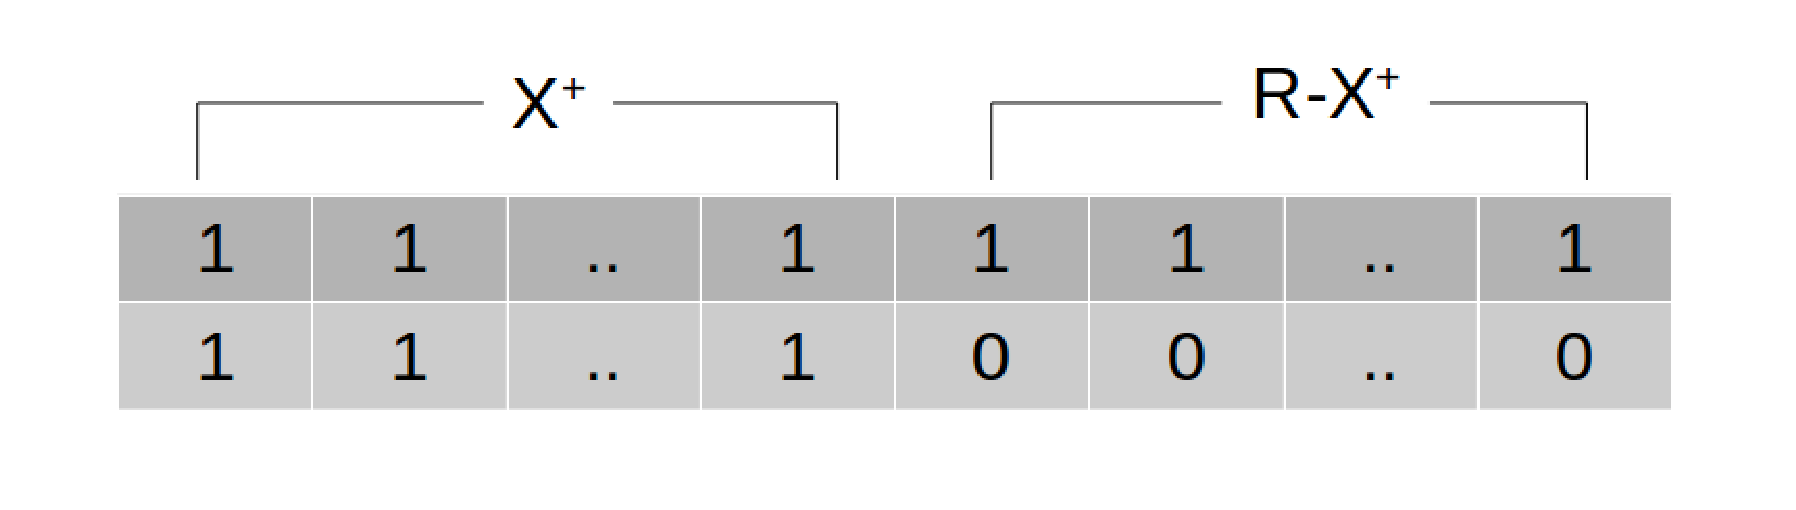
\includegraphics[width=250px]{img_4_4_2.eps} 
\end{center}
Mostriamo che:
\begin{itemize}
 \item $r$ è un'istanza legale di $R$. Sia $V \rightarrow W$ una dipendenza funzionale in $F$ e supponiamo
 per assurdo che non sia soddisfatta da $r$. In tal caso le due tuple di $r$ devono avere gli stessi valori
 per $V$ e differenti valori per $W$; ciò implica che $V \subseteq X^+$ e $W \cap (R-X^+)\not = \emptyset$.
 Poiché $V \subseteq X^+$, per il \linkto{lemma4_1}{Lemma 4.1}, si ha che $X \rightarrow V \in F^A$; pertanto,
 per l'assioma della transitività, $X \rightarrow W \in F^A$ e, quindi, per il Lemma 4.1,
 $W \subseteq X^+$ (che contraddice $W \cap (R-X^+)\not =\emptyset$).
 \item $r$ non soddisfa $X \rightarrow Y$. Supponiamo per assurdo che $r$ soddisfi $X \rightarrow Y$. Poiché 
 $X \subseteq X^+$ (per l'assioma della riflessività), le due tuple di $r$ coincidono sugli attributi $X$ 
 e quindi, poiché $r$ soddisfa $X \rightarrow Y$, devono coincidere anche sugli attributi $Y$. Questo implica
 che $Y \subseteq X^+$ e quindi, per il Lemma 4.1, che $X \rightarrow Y \in F^A$. \hfill $\Box$
\end{itemize}

\subsubsection{Algoritmo per calcolare $X^+$}
Per stabilire se una decomposizione preserva $F^+$, quest'ultimo va calcolato. Tale operazione potrebbe 
tuttavia richiedere tempo esponenziale dipendente da $|F|$; se $F = \{A \rightarrow B_1, A \rightarrow B_2,
\ldots, A \rightarrow B_n\}$, con $|F|=n$, per le regole della decomposizione e dell'unione si ha che 
$F^+ \supseteq \{A \rightarrow Z\ t.c.\ Z \subseteq B_1B_2\ldots B_n\}$ e quindi $|F^+| = 2^n-1$. D'altra parte,
per sapere se una decomposizione preserva le dipendenze, è sufficiente poter decidere se una dipendenza 
funzionale $X \rightarrow Y \in F^+$; ciò può essere fatto calcolando $X^+$ e verificando se $Y \subseteq 
X^+$.\\ 
Il calcolo di $X^+$ può essere fatto mediante il seguente algoritmo polinomiale.
\begin{alg}
\textsc{Input:} uno schema di relazione $R$, un insieme $F$ di dipendenze funzionali su $R$, un sottoinsieme
$X$ di $R$.\\
\textsc{Output:} $X^+_F$ nella variabile $Z$\\\\
\textsc{Begin}\\
$Z\vcentcolon= X$;\\
$S\vcentcolon= \{A\ t.c.\ (Y \rightarrow V \in F) \wedge (A \in V) \wedge (Y \subseteq Z)\}$;\\
\textsc{while} $S \not \subseteq Z$\\
\indent \textsc{begin}\\
\indent $Z\vcentcolon = Z \cup S$;\\
\indent $S\vcentcolon= \{A\ t.c.\ (Y \rightarrow V \in F) \wedge (A \in V) \wedge (Y \subseteq Z)\}$;\\
\indent \textsc{end}\\
\textsc{end}\\
\end{alg}
\begin{exmp}
 Ecco un esempio di esecuzione di tale algoritmo. Sia $R = ABCDEHL$ ed $F=\{A\rightarrow B$, $BC\rightarrow D$,
 $D\rightarrow HL$, $E\rightarrow D\}$. $X=A$.\\\\
 Passo 0: $Z^{(0)}=A$ e $S^{(0)}=B$ \\
 Passo 1: $Z^{(1)}=AB$ mentre $S$ rimane lo stesso.\\
 L'algoritmo termina e $X^+=A^+=AB$.
\end{exmp}

\begin{theo}
L'Algoritmo 4.1 calcola correttamente la chiusura di un insieme di attributi $X$ rispetto ad un insieme $F$ 
di dipendenze funzionali.
\end{theo}
\textbf{Dimostrazione.} Si indichi con $Z^{(0)}$ il valore iniziale di $Z$ (ovvero $Z^{(0)} = X$) e con 
$Z^{(i)}$ ed $S^{(i)}$, $i \geq 1$, i valori di $Z$ ed $S$ dopo l'$i$-esima esecuzione del corpo del ciclo; 
\`e facile vedere che $Z^{(i)} \subseteq Z^{(i+1)}$, $\forall i$. Sia $j$ tale che $S^{(j)} \subseteq Z^{(j)}$
(cio\`e $Z^{(j)}$ \`e il valore di $Z$ quando l'algoritmo termina); si proverà che:
\begin{center}
 \begin{math}
   A \in X^+ \Leftrightarrow A \in Z^{(j)}
 \end{math}
\end{center}
\emph{\textbf{Parte solo se.}} Verrà dimostrato per induzione su $i$ che $Z^{(i)} \subseteq X^+$, $\forall i$, 
e quindi, in particolare $Z^{(j)} \subseteq X^+$.\\
\emph{Base dell'induzione}: $i=0$. Poiché $Z^{(0)} = X$ e $X\subseteq X^+$, si ha $Z^{(0)} \subseteq X^+$.\\
\emph{Induzione}: $i>0$. Per l'ipotesi induttiva $Z^{(i-1)} \subseteq X^+$. Sia $A$ un attributo in $Z^{(i)}
-Z^{(i-1)}$; deve esistere una dipendenza $Y \rightarrow V \in F$ tale che $Y\subseteq Z^{(i-1)}$ e $A \in V$.
Poiché $Y \subseteq Z^{(i-1)}$, per l'ipotesi induttiva si ha che $Y \subseteq X^+$; pertanto, per il 
\linkto{lemma4_1}{Lemma 4.1}, $X \rightarrow Y \in F^A$. Poiché $X \rightarrow Y \in F^A$ e $Y \rightarrow V
\in F$, per l'assioma della transitività si ha $X \rightarrow V \in F^A$ e quindi, per il Lemma 4.1, $V 
\subseteq X^+$. Pertanto, $\forall A \in Z^{(i)} -Z^{(i-1)}$ si ha $A \in X^+$. Da ciò segue, per l'ipotesi 
induttiva, che $Z^{(i)} \subseteq X^+$.\\
\emph{\textbf{Parte se.}} Sia $A$ un attributo in $X^+$. Mostreremo che $A \in Z^{(j)}$. Poiché $A \in X^+$,
si ha $X \rightarrow A \in F^+$ (per il \linkto{teorema4_3}{Teorema 4.3}); pertanto $X \rightarrow A$ deve 
essere soddisfatta da ogni istanza legale di $R$. Si consideri la seguente istanza $r$ di $R$:
\begin{center}
 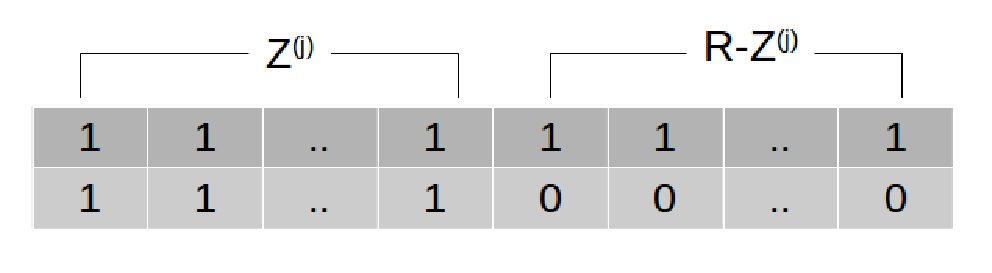
\includegraphics[width=250px]{img_4_4_3.eps}
\end{center}
Mostriamo che $r$ è un'istanza legale di $R$. Infatti, se, per assurdo, esistesse in $F$ una dipendenza
funzionale $V \rightarrow W$ non soddisfatta da $r$, si dovrebbe avere $V \subseteq Z^{(j)}$ e $W \cap 
(R-Z^{(j)})\not = \emptyset$; ma, in tal caso, si avrebbe $S^{(j)} \not \subseteq Z^{(j)}$ (contraddizione).
Poiché $r$ è un'istanza legale di $R$ deve soddisfare $X \rightarrow A$; ma, allora, poiché $X = Z^{(0)} 
\subseteq Z^{(j)}$, $A$ deve essere in $Z^{(j)}$.\hfill $\Box$\\

Tramite l'\textsc{Algoritmo 4.1} possiamo verificare se un insieme di attributi è una chiave valida per
uno schema di relazione; basta verificare, per la sua \linkto{defn_4_3}{Definizione 4.3} e per il \linkto{lemma4_1}{Lemma 4.1},
che la sua chiusura rispetto ad $F$ includa o sia uguale alla relazione e che non lo siano le chiusure
dei suoi sottoinsiemi. Vediamo un esempio.
\begin{exmp}
Sia $R=ABCDEH$ ed $F=\{AB\rightarrow CD$, $C\rightarrow DE$, $E\rightarrow AC\}$. Mostrare che:
\begin{itemize}
 \item $ABH$ è chiave per $R$;
 \item sapendo che è l'unica chiave di $R$, dire perché $R$ non è in 3NF.
\end{itemize}

\noindent \textbf{Soluzione.}\\
$(ABH)^+_F = ABCDEH = R$ e inoltre\\
$(AB)^+_F = ABCDE \not= R$\\
$(AH)^+_F = AH \not= R$\\
$(HB)^+_F = HB \not= R$\\

Ne tantomeno lo saranno le chiusure dei singoli attributi. Quindi abbiamo dimostrato che $ABH$ è chiave di $R$.\\
La relazione $R$ non è in 3NF perché contiene dipendenze parziali e transitive:
\begin{itemize}
 \item $AB\rightarrow CD$ è una dipendenza parziale;
 \item $C\rightarrow DE$, $E\rightarrow AC$ sono dipendenze transitive;
\end{itemize}
e ciò va contro la definizione di schema in Terza Forma Normale.
\end{exmp}


\subsection{Decomposizioni che preservano le dipendenze funzionali}
Si vuole ora formalizzare il concetto di decomposizione che ``preserva un insieme di dipendenze funzionali''.
A tal fine, cominciamo con l'introdurre i concetti di \emph{decomposizione} di uno schema di relazione ed 
\emph{equivalenza} tra due insiemi di dipendenze funzionali.\\
\begin{defn}
Sia $R$ uno schema di relazione. Una \textbf{decomposizione} di $R$ è una famiglia $\rho = \{R_1, R_2, \ldots, 
R_k\}$ di sottoinsiemi di $R$ che \emph{ricopre} $R$ ($\bigcup_{i=1}^k R_i = R$).
\end{defn}
\begin{exmp}
Sia $R = ABC$. Le decomposizioni $\{AB, BC\}$ e $\{A, BC\}$ sono valide, mentre non lo è $\{AB, B\}$ poiché
manca l'attributo $C$.
\end{exmp}

\subsubsection{Equivalenza tra due insiemi di dipendenze funzionali}
\begin{defn}
Siano $F$ e $G$ due insiemi di dipendenze funzionali. $F$ e $G$ sono \textbf{equivalenti}, in simboli $F \equiv 
G$, se $F^+ = G^+$.
\end{defn}
Verificare l'equivalenza di due insiemi $F$ e $G$ di dipendenze funzionali richiede dunque che venga verificata
l'uguaglianza di $F^+$ e $G^+$, cioè che $F^+ \subseteq G^+$ e contemporaneamente $F^+ \supseteq G^+$. Come 
detto in precedenza, calcolare la chiusura di un insieme di dipendenze funzionali può richiedere tempo 
esponenziale. Il seguente lemma ci permette tuttavia di verificare l'equivalenza dei due insiemi di dipendenze
funzionali in tempo polinomiale.
\label{lemma4_2}
\begin{lem}
Siano $F$ e $G$ due insiemi di dipendenze funzionali. $F \subseteq G^+ \Rightarrow F^+ \subseteq G^+$. 
\end{lem}
\textbf{Dimostrazione.} Sia $f \in (F^+ -F)$. Poiché, per il \linkto{teorema4_3}{Teorema 4.3}, $f$ è derivabile
da $F$ mediante gli assiomi di Armstrong e ogni dipendenza funzionale in $F$ è derivabile da $G$ mediante gli 
assiomi di Armstrong, $f$ è derivabile da $G$ mediante gli assiomi di Armstrong. \hfill $\Box$

\begin{defn}
Sia $R$ uno schema di relazione, $F$ un insieme di dipendenze funzionali su $R$ e $\rho = \{R_1, R_2, \ldots,
R_k\}$ una decomposizione di $R$. Diciamo che $\rho$ \emph{preserva} $F$ se $F \equiv \bigcup_{i=1}^k 
\pi_{R_i}(F)$, dove $\pi_{R_i}(F) = \{X \rightarrow Y\ t.c.\ X \rightarrow Y \in F^+ \wedge XY \subseteq R_i\}$.
\end{defn}

\begin{exmp}
 Riprendiamo i dati dell'\linkto{esempio_4_2}{Esempio 4.2}: la relazione $Studente = \{Matr, Com, Prov\}$,
 con $F = $ \{$Matr\rightarrow Com$, $Matr\rightarrow Prov$, $Com\rightarrow Prov$\}. Una decomposizione possibile
 individuata precendentemente è:
  \begin{center}
    $R_1 = \{Matr, Com\}$ con $F_1 = \{Matr\rightarrow Com\}$ \\
    $R_2 = \{Matr, Prov\}$ con $F_2 = \{Matr\rightarrow Prov\}$ \\
   \end{center}
 Si verifica applicando la definizione 4.10 che la dipendenza $Com \rightarrow Prov$ non è preservata, 
 perché in $R_1$ manca $Prov$ e in $R_2$ manca $Com$. Una scelta alternativa per $R_2$ è
 $\{Com, Prov\}$; in questo modo tutte le dipendenze funzionali sono preservate. In altre parole abbiamo
 \textbf{proiettato le dipendenze}, ovvero abbiamo preso gli insiemi di attributi $X$ e $Y$ da una dipendenza funzionale
 $X \rightarrow Y$ e vedere se essi sono presenti nella relazione esaminata.
\end{exmp}


\subsubsection{Algoritmo per verificare l'equivalenza tra F e G}
Verificare se una decomposizione preserva un insieme di dipendenze funzionali $F$ richiede, dunque,
che venga verificata l'equivalenza dei due insiemi di dipendenze funzionali $F$ e $G = \bigcup_{i=1}^k
\pi_{R_i}(F)$; poiché, per definizione, $F^+ \supseteq G$, per il \linkto{lemma4_2}{Lemma 4.2} è sufficiente
verificare che $F\subseteq G^+$; ciò può essere fatto con il seguente algoritmo (la cui correttezza è una 
banale conseguenza del \linkto{lemma4_1}{Lemma 4.1} e del \linkto{teorema4_3}{Teorema 4.3}).

\begin{alg}
\textsc{Input:} due insiemi $F$ e $G$ di dipendenze funzionali su $R$;\\
\textsc{Output:} la variabile \emph{successo} che avrà valore \textsc{true} se $F\subseteq G^+$, \textsc{false}
altrimenti;\\
\textsc{Begin}\\
$successo\vcentcolon=\ true$;\\
\textsc{for each} $X \rightarrow Y \in F$\\
\indent \textsc{begin}\\
\indent $calcola\ X_{G}^+$;\\
\indent \textsc{if} $Y \not\subseteq X^+_G$ \textsc{then} $successo=false$;\\
\indent \textsc{end}\\
\textsc{end}
\end{alg}

\noindent L'\textsc{Algoritmo 2} richiede che venga calcolato $X^{+}_G$; se si volesse utilizzare a tale scopo l'\textsc{Algoritmo 1}
si dovrebbe prima calcolare $G$, ma, per la definizione di $G$, ciò richiederebbe il calcolo di $F^+$ che
richiede tempo esponenziale. Il seguente algoritmo permette di calcolare $X^{+}_G$ a partire da $F$.

\begin{alg}
\textsc{Input}: uno schema di relazione $R$, un insieme $F$ di dipendenze funzionali su $R$, una
decomposizione $\rho =\{R_1, R_2, \ldots, R_k\}$ di $R$, un sottoinsieme $X$ di $R$;\\
\textsc{Output}: la chiusura di $X$ rispetto a $G = \bigcup_{j=1}^k \pi_{R_j}(F)$, (nella variabile $Z$);\\\\
\textsc{Begin}
$Z\vcentcolon = X$;\\
$S\vcentcolon = \emptyset$;\\
\textsc{for} $j\vcentcolon = 1$ \textsc{to} $k$\\
\indent$S \vcentcolon= S \cup [(Z \cap R_j)^{+}_F \cap R_j]$;\\
\textsc{while} $S \not\subseteq Z$\\
\indent \textsc{Begin}\\
\indent $Z\vcentcolon = Z \cup S$;\\
\indent \textsc{for} $j\vcentcolon= 1$ \textsc{to} $k$\\
\indent \indent $S\vcentcolon= S \cup [(Z \cap R_j)^{+}_F \cap R_j]$;\\
\indent \textsc{end}\\
\textsc{end}\\
\end{alg}
\begin{exmp}
Dato $R=ABCDEH$, $F=\{AB\rightarrow CD$, $E \rightarrow H$, $CD\rightarrow E$, $H\rightarrow AB\}$ ed una scomposizione
di $R$, $\rho=\{ABCD$, $CDEH\}$. $\rho$ preserva $F$?\\

\noindent \textbf{Soluzione.}\\
Prendiamo la prima dipendenza funzionale in $F$, $AB\rightarrow CD$. Notiamo che $AB \cup CD$ è presente in una delle due
relazioni della scomposizione, quindi tale dipendenza funzionale è per certo facente parte di $G^+$. Lo stesso vale per
$E\cup H$, $CD\cup E$. Rimane solo da verificare $H\rightarrow AB$ tramite l'algoritmo.\\\\
$Z^{(0)}= H$;\\
$S^{(0)} = (H \cap ABCD)^+_F \cap ABCD = \emptyset$;\\
$S^{(1)} = S^{(0)} \cup (H \cap CDEH)^+_F \cap CDEH = \emptyset \cup CDEH$;\\\\
Dato che $S\not\subseteq Z$ eseguiamo il ciclo \textsc{while}:\\\\
$Z^{(1)}= CDEH$;\\
Entriamo nel for:\\
\indent $S^{(2)} = S^{(1)} \cup [(CDEH \cap ABCD)^+_F \cap ABCD] = ABCDEH$;\\
\indent $S^{(3)} = S^{(2)} \cup [(CDEH \cap CDEH)^+_F \cap CDEH] = ABCDEH$;\\

\noindent Terminato il ciclo for notiamo che un'altra volta $S\not\subseteq Z$, quindi rieseguiamo il ciclo while:\\\\
$Z^{(2)}= ABCDEH$;\\
entriamo nel for:\\
\indent $S^{(4)} = S^{(3)} \cup [(ABCDEH \cap ABCD)^+_F \cap ABCD] = ABCDEH$;\\
\indent $S^{(5)} = S^{(4)} \cup [(ABCDEH \cap CDEH)^+_F \cap CDEH] = ABCDEH$;\\

\noindent Notiamo che essenzialmente $S$ non è cambiato ma $Z$ si, quindi ora $S \subseteq Z$ e si 
esce dal ciclo \textsc{while} per tornare all'Algoritmo 1. $H \subseteq ABCDEH$ 
quindi la variabile \emph{successo} rimane uguale a \emph{true}. Troviamo quindi che: 
$AB\rightarrow CD \in G^+$, $E \rightarrow H  \in G^+$, 
$CD\rightarrow E \in G^+$, $H\rightarrow AB  \in G^+$. Ne segue $\rho$ preserva $R$.
\end{exmp}

\begin{theo}
Sia $R$ uno schema di relazione, $F$ un insieme di dipendenze funzionali su $R$, $\rho =\{R_1, R_2, \ldots, R_k\}$
una decomposizione di $R$ e $X$ un sottoinsieme di $R$. L'Algoritmo 4.3 calcola correttamente $X^{+}_G$, dove 
$G = \bigcup_{j=1}^k \pi_{R_j}(F)$.
\end{theo}
\textbf{Dimostrazione.} Indichiamo con $Z^{(0)}$ il valore iniziale di $Z$ ($Z^{(0)} = X$) e con $Z^{(i)}$, $i \geq 
1$, il valore di $Z$ dopo l'$i$-esima esecuzione dell'assegnazione $Z \vcentcolon= Z \cup S$; è facile vedere che 
$Z^{(i)} \subseteq Z^{(i+1)}$, $\forall i$. Sia $Z^{(f)}$ il valore di $Z$ quando l'algoritmo termina; proveremo che:
\begin{center}
\begin{math}
  A \in X^{+}_G \Leftrightarrow  A \in Z^{(f)} 
\end{math}
\end{center}
\textbf{\emph{Parte solo se.}} Mostreremo per induzione su $i$ che $Z^{(i)} \subseteq X^{+}_G$, $\forall i$.\\
\emph{Base dell'induzione}: $i=0$. Poiché $Z^{(0)} = X$ e $X \subseteq X^+$, si ha $Z^{(0)} \subseteq X^{+}_G$.\\
\emph{Induzione}: $i >0$. Per l'ipotesi induttiva $Z^{(i-1)} \subseteq X^{+}_G$. Sia $A$ un attributo in $Z^{(i)}
-Z^{(i-1)}$; in tal caso deve esistere un indice $j$ tale che $A \in (Z^{(i-1)} \cap R_j)^{+}_F \cap R_j$. Poiché
$A \in (Z^{(i-1)} \cap R_j)^{+}_F$ si ha $(Z^{(i-1)} \cap R_j) \rightarrow A \in F^+$ (per il Teorema 4.3).\\
Poiché $(Z^{(i-1)} \cap R_j) \rightarrow A \in F^+$, $A \in R_j$ e $Z^{(i-1)} \cap R_j \subseteq R_j$ si ha, per 
la definizione di $G$, che $(Z^{(i-1)} \cap R_j) \rightarrow A \in G$. Poiché per l'ipotesi induttiva si ha che 
$X \rightarrow Z^{(i-1)} \in G^+$, per la regola di decomposizione si ha anche che $X \rightarrow (Z^{(i-1)} 
\cap R_j) \in G^+$ e, quindi, per l'assioma della transitività, che $X \rightarrow A \in G^+$, cioè $A \in X^{+}_G$.
Quindi $Z^{(i)} \subseteq X^{+}_G$.\\
\textbf{\emph{Parte se.}} Mostreremo che $X^{+}_G \subseteq Z^{(f)}$ tenendo conto anche della seguente proposizione:
\begin{prop}
Presi comunque due insiemi di attributi $X$ ed $Y$ e un insieme di dipendenze funzionali $F$ si ha, per la 
definizione di chiusura di un insieme di attributi, $X \subseteq Y \Rightarrow X^{+}_F \subseteq Y^{+}_F$. 
\end{prop}
Poichè $X = Z^{(0)} \subseteq Z^{(f)}$, dalla Proposizione 4.4 segue che $X^{+}_G \subseteq (Z^{(f)})^{+}_G$. 
Mostreremo che $Z^{(f)} = (Z^{(f)})^+_G$ da cui segue $X^+_G \subseteq Z^{(f)}.$\\
Supponiamo per assurdo che $Z^{(f)}\not =(Z^{(f)})^+_G$. Consideriamo l'\textsc{Algoritmo 4.1} che, per evitare ambiguità,
riscriviamo sostituendo la variabile $W$ alla variabile $Z$ e la variabile $U$ alla variabile $S$:\\

\noindent\textsc{Input:} uno schema di relazione $R$, un insieme $F$ di dipendenze funzionali su $R$, un sottoinsieme
$X$ di $R$.\\
\textsc{Output:} $X^+_F$ nella variabile $W$\\\\
\textsc{Begin}\\
$W\vcentcolon= X$;\\
$U\vcentcolon= \{A\ t.c.\ (Y \rightarrow V \in F) \wedge (A \in V) \wedge (Y \subseteq W)\}$;\\
\textsc{while} $U \not \subseteq W$\\
\indent \textsc{begin}\\
\indent $W\vcentcolon = W \cup U$;\\
\indent $U\vcentcolon= \{A\ t.c.\ (Y \rightarrow V \in F) \wedge (A \in V) \wedge (Y \subseteq W)\}$;\\
\indent \textsc{end}\\
\textsc{end}\\

Se eseguiamo tale algoritmo fornendo in input l'insieme di attributi $Z^{(f)}$ e l'insieme di dipendenze 
funzionali $G$, al termine la variabile $W$ conterrà $(Z^{(f)})^+_G$. Se, come abbiamo supposto per assurdo,
$Z^{(f)}\not =(Z^{(f)})^+_G$, deve esistere un attributo $B$ che appartiene a $U^{(0)}$ e non appartiene 
a $W^{(0)} =Z^{(f)}$ (altrimenti si avrebbe $Z^{(f)} =(Z^{(f)})^+_G$). D'altra parte si ha:
\begin{center}
\begin{math}
U^{(0)} = \{A\ t.c.\ (Y \rightarrow V \in G) \wedge (A \in V) \wedge (Y \subseteq W^{(0)})\}
\end{math}
\end{center}
e quindi, per la definizione di $G$, deve esistere $j$ tale che:
\begin{center}
 \begin{math}
  B \in \{A\ t.c.\ (Y \rightarrow V \in F^+) \wedge (A \in V) \wedge (Y \subseteq W^{(0)}) \wedge (YV \subseteq R_j)\}
 \end{math}
\end{center}
Da $Y \subseteq W^{(0)} \wedge YV \subseteq R_j$ segue che:
\begin{center}
 \begin{math}
  [a]\ Y \subseteq W^{(0)} \cap R_j = Z^{(f)} \cap R_j
 \end{math}
\end{center}
Inoltre dal fatto che $Y \rightarrow V \in F^+$ segue, per il \linkto{lemma4_1}{Lemma 4.1}, che $V \subseteq Y^+_F$
e, quindi, per la [a] e per la Proposizione 4.4 si ha che $V \subseteq (Z^{(f)} \cap R_j)^+_F$. Infine 
poichè $YV \subseteq R_j$ si ha:
\begin{center}
 \begin{math}
 V \subseteq (Z^{(f)} \cap R_j)^+_F \cap R_j
 \end{math}
\end{center}
Poiché $B \in V$ si ha che $B \in (Z^{(f)} \cap R_j)^+_F \cap R_j$ e quindi $B \in S^{(f)}$. Poiché $B$ non 
appartiene a $Z^{(f)}$ (per l'ipotesi per assurdo), $Z^{(f)}$ non può essere il valore finale di $Z$ 
(contraddizione). \hfill $\Box$

\subsection{Decomposizioni con Join senza perdita}

Come è stato ribadito nel paragrafo 4.3, se si decompone uno schema di relazione $R$ che non è in 3NF si
vuole che la decomposizione $\{R_1, R_2, \ldots, R_k\}$ ottenuta sia tale che ogni istanza legale $r$
di $R$ sia ricostruibile mediante join naturale (il cui simbolo ricordiamo essere $\bowtie$) da un istanza 
legale $\{r_1, r_2, \ldots, r_k\}$ dello schema decomposto $\{R_1, R_2, \ldots, R_k\}$. Poiché per ricostruire
una tupla $t$ di $r$ è necessario che $t[R_i] \in R_i$, $\forall i \in \{1, \ldots, k\}$, si deve avere $r_i =
\pi_{R_i}(r)$, $\forall i \in \{1, \ldots, k\}$.
\begin{defn}
Sia $R$ uno schema di relazione. Una decomposizione $\rho = \{R_1, R_2, \ldots, R_k\}$ di $R$ ha un
\emph{join senza perdita} se per ogni istanza legale $r$ di $R$ si ha $r = \pi_{R_1}(r) \bowtie \pi_{R_2}(r) 
\bowtie \ldots \bowtie \pi_{R_k}(r)$.
\end{defn}
\begin{theo}
Sia $R$ uno schema di relazione e $\rho = \{R_1, R_2, \ldots, R_k\}$ una decomposizione di $R$. Per ogni
istanza legale $r$ di $R$, indicato con $m_{\rho}(r) =\pi_{R_1}(r) \bowtie \pi_{R_2}(r) 
\bowtie \ldots \bowtie \pi_{R_k}(r)$, si ha:
\begin{enumerate}
 \item $r\subseteq m_{\rho}(r)$
 \item $\pi_{R_i}(m_{\rho}(r)) = \pi_{R_i}(r)$
 \item $m_{\rho}(m_{\rho}(r)) = m_{\rho}(r)$
\end{enumerate}
\end{theo}
\textbf{Dimostrazione.}\\
\emph{Prova di }[1]. Sia $t$ una tupla di $r$. $\forall i \in \{1, \ldots, k\}$, $t[R_i] \in \pi_{R_i}(r)$ e
quindi $t \in m_{\rho}(r)$.\\
\emph{Prova di }[2]. Per il punto [1] si ha $r \subseteq m_{\rho}(r)$ e, quindi, $\pi_{R_i}(r) \subseteq 
\pi_{R_i}(m_{\rho}(r))$. E' sufficiente, pertanto, mostrare che $\pi_{R_i}(r) \supseteq \pi_{R_i}(m_{\rho}(r))$.
Banalmente, per ogni tupla $t \in m_\rho(r)$ e per ogni $i \in \{1, \ldots, k\}$, deve esistere una tupla
$t' \in r\ t.c.\ t[R_i] = t'[R_i]$.\\
\emph{Prova di }[3]. Per il punto [2] si ha $\pi_{R_i}(m_\rho(r)) = \pi_{R_i}(r)$. Pertanto
\begin{center}
$m_\rho(m_\rho(r)) = \pi_{R_1}(m_\rho(r)) \bowtie \ldots \bowtie \pi_{R_k}(m_\phi(r)) = \pi_{R_1}(r) \bowtie
\ldots \bowtie \pi_{R_k}(r) = m_\rho(r)$. 
\end{center}
\hfill $\Box$\\\\
Il seguente algoritmo permette di decidere in tempo polinomiale se una decomposizione di uno schema di relazione
ha un join senza perdita.

\begin{alg}
 \textsc{Input}: uno schema di relazione $R$, un insieme $F$ di dipendenze funzionali su $R$, una decomposizione
 $\rho = \{R_1, R_2, \ldots, R_k\}$ di $R$;\\
 \textsc{Output}: decide se $\rho$ ha un join senza perdita;\\\\
 \textsc{Begin}\\
 Costruisci una tabella $r$ nel modo seguente:
 \begin{itemize}
  \item $r$ ha $|R|$ colonne e $|\rho|$ righe
  \item all'incrocio dell'$i$-esima riga e della $j$-esima colonna si metta:
  \begin{itemize}
   \item il simbolo $a_j$ se l'attributo $A_j \in R_i$;
   \item il simbolo $b_{i,j}$ altrimenti;
  \end{itemize}
 \end{itemize}
 \textsc{repeat}\\
 \indent \textsc{for each} $X\rightarrow Y \in F$\\
 \indent \indent \textsc{do}\\
 \indent \indent \textsc{if} $\exists \{t_1, t_2\} \in r\ t.c.\ t_1[X]=t_2[X] \wedge t_1[Y]\not= t_2[Y]$ \textsc{then}\\
 \indent \indent \indent \textsc{for each} $A_j \in Y$\\
 \indent \indent \indent \indent \textsc{if} $t_1[A_j]=`a_j\text{'}$ \textsc{then} $t_2[A_j]\vcentcolon= t_1[A_j]$;\\
 \indent \indent \indent \indent \textsc{else} $t_1[A_j]\vcentcolon= t_2[A_j]$;\\\\
 \textsc{until} $r$ ha una riga con tutte `a' \textsc{or} $r$ non è cambiato;\\
 \textsc{if} $r$ ha una riga con tutte `a' \textsc{then}\\
 \indent $\rho$ ha un join senza perdita;\\
 \textsc{else}\\
 \indent $\rho$ non ha un join senza perdita;\\
 \textsc{end}\\
\end{alg}

Il seguente esempio mostra come tale algorimo viene applicato.\\
\begin{exmp}
 Sia $R=ABCDEH$ uno schema di relazione, $F=\{C\rightarrow D,\ DH\rightarrow C,\ D\rightarrow H,\ A \rightarrow BC\}$
 un insieme di dipendenze funzionali su $R$ e $\rho = \{AE, ABDH, CDE\}$ una scomposizione di $R$. Quello che 
 vogliamo sapere è: $\rho$ ha un join senza perdita?\\
 Come indicato dall'Algoritmo 4.4, si costruisca una tabella che ha come colonne gli attributi di $R$ e come 
 righe le varie relazioni in $\rho$, inserendo poi in ogni cella uno dei due simboli indicati nell'algoritmo,
 secondo il criterio specificato. Nella cella individuata dalla prima colonna e dalla prima riga, ad esempio, 
 va messo il simbolo $a_1$ visto che l'attributo $A$ rappresentante la \emph{prima} colonna è presente nella 
 relazione rappresentante la prima riga; nella seconda colonna, prima riga, la cella contiene $b_{1,2}$ poiché
 $B$ non è presente in $AE$.
 \begin{center}
  \begin{tabular}{c|c|c|c|c|c|c}
    & \textbf{A} & \textbf{B} &\textbf{C}&\textbf{D}&\textbf{E}&\textbf{H}\\
   \hline
   \textbf{AE} & $a_1$ & $b_{1,2}$ & $b_{1,3}$ & $b_{1,4}$ & $a_5$ & $b_{1,6}$\\
   \hline
   \textbf{ABDH}& $a_1$ & $a_2$ & $b_{2,3}$ & $a_4$ & $b_{2,5}$ & $a_6$\\
   \hline
   \textbf{CDE} & $b_{3,1}$ & $b_{3,2}$ & $a_3$ & $a_4$ & $a_5$ & $b_{3,6}$\\
  \end{tabular}
 \end{center}
 
 Ora, per ogni dipendenza funzionale $A\rightarrow Y \in F$, controlliamo se ci sono due righe (tuple) $t_1$
 e $t_2$ tali che $t_1[X] = t_2[X]$ e $t_1[Y] \not= t_2[Y]$. In questo caso abbiamo le dipendenze funzionali $D\rightarrow H$ e 
 $A \rightarrow BC$ verifica tale condizione; per convenienza conviene segnare, ad ogni iterazione dell'algoritmo, quali 
 dipendenze funzionali verifichino la suddetta condizione. Usiamo la seguente tabella dove le colonne sono le iterazioni, 
 e le righe rappresentano le dipendenze funzionali. Inseriremo una ``$\checkmark$'' quando una dipendenza funzionale 
 verifica la condizione; ``$\cdot$'' altrimenti:\\
 \begin{center}
  \begin{tabular}{l|c|}
   & $I_1$\\
   \hline
   $C\rightarrow D$ & $\cdot$\\
   $DH\rightarrow C$& $\cdot$\\
   $D \rightarrow H$ & $\checkmark$\\
   $A \rightarrow BC$ & $\checkmark$\\
  \end{tabular}
 \end{center}
 
 Tornando alla tabella precedente, visto che l'ultima dipendenza funzionale verifica la condizione cercata nelle righe 1 e 2,
 andiamo a modificare i valori di ogni attributo $Y$, in questo caso $Y= BC$; dato che $t_1[B]\not= a_j$ abbiamo che il valore
 della cella diviene uguale a $t_2[B]$, mentre $t_1[C]\vcentcolon= t_2[C]$. Dopo queste modifiche, al termine della \textbf{prima 
 iterazione} si ha la seguente situazione:
 \begin{multicols}{2}
   \begin{center}
  \begin{tabular}{c|c|c|c|c|c|c}
    & \textbf{A} & \textbf{B} &\textbf{C}&\textbf{D}&\textbf{E}&\textbf{H}\\
   \hline
   \textbf{AE} & $a_1$ & $\mathbf{a_2}$ & $\mathbf{b_{2,3}}$ & $b_{1,4}$ & $a_5$ & $b_{1,6}$\\
   \hline
   \textbf{ABDH}& $a_1$ & $a_2$ & $b_{2,3}$ & $a_4$ & $b_{2,5}$ & $a_6$\\
   \hline
   \textbf{CDE} & $b_{3,1}$ & $b_{3,2}$ & $a_3$ & $a_4$ & $a_5$ & $\mathbf{a_6}$\\
  \end{tabular}
 \end{center}
 
  \begin{center}
  \begin{tabular}{l|c}
   & $I_1$\\
   \hline
   $C\rightarrow D$ & $\cdot$\\
   $DH\rightarrow C$& $\cdot$\\
   $D \rightarrow H$ & $\checkmark$\\
   $A \rightarrow BC$ & $\checkmark$\\
  \end{tabular}
 \end{center}
 \end{multicols}
L'algoritmo non ha terminato la sua esecuzione perché non ha riscontrato una condizione di uscita (una riga con tutte ``a'' o
l'ultima iterazione eseguita non ha apportato nessun cambiamento). Procediamo quindi con le successive iterazioni.\\

\textbf{Iterazione 2}
 \begin{multicols}{2}
   \begin{center}
  \begin{tabular}{c|c|c|c|c|c|c}
    & \textbf{A} & \textbf{B} &\textbf{C}&\textbf{D}&\textbf{E}&\textbf{H}\\
   \hline
   \textbf{AE} & $a_1$ & $a_2$ & $b_{2,3}$ & $\mathbf{a_4}$ & $a_5$ & $b_{1,6}$\\
   \hline
   \textbf{ABDH}& $a_1$ & $a_2$ & $\mathbf{a_3}$ & $a_4$ & $b_{2,5}$ & $a_6$\\
   \hline
   \textbf{CDE} & $b_{3,1}$ & $b_{3,2}$ & $a_3$ & $a_4$ & $a_5$ & $a_6$
  \end{tabular}
 \end{center}
 
  \begin{center}
  \begin{tabular}{l|c|c}
   & $I_1$ & $I_2$\\
   \hline
   $C\rightarrow D$& $\cdot$ & $\checkmark$\\
   $DH\rightarrow C$& $\cdot$& $\checkmark$\\
   $D \rightarrow H$& $\checkmark$ & $\cdot$\\
   $A \rightarrow BC$& $\checkmark$ & $\cdot$
  \end{tabular}
 \end{center}
 \end{multicols}
\textbf{Iterazione 3}
 \begin{multicols}{2}
   \begin{center}
  \begin{tabular}{c|c|c|c|c|c|c}
    & \textbf{A} & \textbf{B} &\textbf{C}&\textbf{D}&\textbf{E}&\textbf{H}\\
   \hline
   \textbf{AE} & $a_1$ & $a_2$ & $\mathbf{a_3}$ & $a_4$ & $a_5$ & $\mathbf{a_6}$\\
   \hline
   \textbf{ABDH}& $a_1$ & $a_2$ & $a_3$ & $a_4$ & $b_{2,5}$ & $a_6$\\
   \hline
   \textbf{CDE} & $b_{3,1}$ & $b_{3,2}$ & $a_3$ & $a_4$ & $a_5$ & $a_6$
  \end{tabular}
 \end{center}
 
  \begin{center}
  \begin{tabular}{l|c|c|c}
   & $I_1$ & $I_2$ & $I_3$\\
   \hline
   $C\rightarrow D$& $\cdot$ & $\checkmark$ & $\cdot$\\
   $DH\rightarrow C$& $\cdot$& $\checkmark$ & $\cdot$\\
   $D \rightarrow H$& $\checkmark$ & $\cdot$ & $\checkmark$\\
   $A \rightarrow BC$& $\checkmark$ & $\cdot$ & $\checkmark$\\
  \end{tabular}
 \end{center}
 \end{multicols}
\noindent Alla fine della terza iterazione ci accorgiamo che la prima riga è composta da soli elementi $a_j$, quindi l'algoritmo
termina indicando che $\rho$ ha un join senza perdita.
 \end{exmp}


\begin{theo}
Sia $R$ uno schema di relazione, $F$ un insieme di dipendenze funzionali su $R$ e $\rho =\{R_1, R_2, \ldots, R_k\}$
una decomposizione di $R$. L'Algoritmo 4.4 decide correttamente se $\rho$ ha un join senza perdita.
\end{theo}
\textbf{Dimostrazione.} Occorre dimostrare che: quando l'algoritmo termina la tabella r ha una tupla con tutte `a' 
$\Leftrightarrow$ $\rho$ ha un join senza perdita. Verrà dimostrata solo la parte ``solo se'' (per uno sketch della 
prova della parte ``se'' consultare il testo di Ullman).\\
\emph{Parte solo se.} Supponiamo per assurdo $\rho$ abbia un join senza perdita e che quando l'algoritmo
termina la tabella $r$ non abbia una tupla con tutte `a'. La tabella $r$ può essere interpretata come
un'istanza legale di $R$ (basta sostituire ai simboli `a' e `b' valori presi dai domini dei corrispondenti
attributi in modo tale che ad uno stesso simbolo venga sostituito lo stesso valore) in quanto
l'algoritmo termina quando non ci sono più violazioni delle dipendenze in $F$. Poiché nessun
simbolo `a' che compare nella tabella costruita inizialmente viene mai modificato dall'algoritmo,
per ogni $i \in \{1, \ldots k\}$, $\pi_{R_i}(r)$ contiene una tupla con tutte `a'; pertanto $m_\rho(r)$ contiene una 
tupla con tutte `a' e, quindi, $m_\rho(r) \not= r$ (contraddizione).
\begin{cor}
Sia $R$ uno schema di relazione, $F$ un insieme di dipendenze funzionali su $R$ e $\rho = \{R_1, R_2\}$
una decomposizione di $R$.
\begin{center}
$(R_1 \cap R_2) \rightarrow (R_1 - R_2) \vee (R_1 \cap R_2) \rightarrow (R_2 -R_1) \Rightarrow \rho$ ha un join senza 
perdita.                            
\end{center}
\end{cor}

\subsection{Decomposizioni in 3NF che conservano la dipendenze funzionali e hanno un join senza perdita}

In questo paragrafo mostreremo che: 
\begin{prop}
Dato uno schema di relazione $R$ e un insieme di dipendenze funzionali $F$ su $R$ esiste sempre una decomposizione
$\rho = \{R_1, R_2, \ldots, R_k\}$ di $R$ tale che:
\begin{itemize}
 \item $\forall i, i \in \{1, \ldots, k\}$, $R_i$ è in 3NF;
 \item preserva $F$;
 \item $\rho$ ha un join senza perdita
\end{itemize}
e che una tale decomposizione può essere calcolata in tempo polinomiale. 
\end{prop}

A tal fine abbiamo bisogno di introdurre il concetto di copertura minimale di un insieme di dipendenze funzionali.
\begin{defn}
Sia $F$ un insieme di dipendenze funzionali. Una \textbf{copertura minimale} di $F$ è un insieme $G$ di dipendenze 
funzionali equivalente ad $F$ tale che:
\begin{enumerate}
 \item per ogni dipendenza funzionale in $G$ la parte destra è un singleton, cioè è costituita da un unico
attributo (ogni attributo nella parte destra è non ridondante);
 \item $\nexists X \rightarrow A \in G\ t.c.\ \exists X' \subseteq X\ t.c.\ G \equiv G - \{X \rightarrow A\} 
 \cup \{X' \rightarrow A\}$ (ogni attributo nella parte sinistra è non ridondante);
 \item $\nexists X \rightarrow A \in G\ t.c.\ G \equiv G - \{X \rightarrow A\}$ (ogni dipendenza è non ridondante). 
\end{enumerate}
\end{defn}
Per ogni insieme di dipendenze funzionali $F$ esiste una copertura minimale che può essere ottenuta in tempo polinomiale
a partire dall'insieme $G$ equivalente ad $F$ in cui per ogni dipendenza funzionale la parte destra è un singleton 
($G$ esiste sempre per la regola della decomposizione)
\begin{itemize}
 \item prima sostituendo ricorsivamente ogni dipendenza funzionale $A_1, \ldots, A_{i-1}, A_i, A_{i+1}, \ldots, A_n 
 \rightarrow A\}$ tale che $G \equiv G - \{A_1, \ldots, A_{i-1}, A_i, A_{i+1}, \ldots, A_n \rightarrow A\} \cup 
 \{A_1, \ldots, A_{i-1}, A_{i+1}, \ldots, A_n \rightarrow A\}$ con la dipendenza funzionale $\{A_1, \ldots, A_{i-1}, A_{i+1},
 \ldots, A_n \rightarrow A\}$
 \item e successivamente eliminando ricorsivamente ogni dipendenza funzionale $X \rightarrow A\ t.c.\ G \equiv G- 
 \{X \rightarrow A\}$.
\end{itemize}
 
 Vediamo ora un'applicazione dell'algoritmo per trovare la copertura minimale di un insieme di dipendenze funzionali.
\begin{exmp}
Sia dato $F = \{AB\rightarrow CD$, $A\rightarrow CH$, $H\rightarrow D\}$. Vogliamo trovare la copertura minimale, chiamiamola $G$, di $F$.\\

\noindent \textbf{Primo passo:} partiamo col trasformare ogni dipendenza che ha più di un attributo a destra in più dipendenze
con un solo attributo a destra. \`E possibile ``sdoppiare'' una dipendenza funzionale grazie alla regola della \emph{decomposizione};
cosi facendo modifichiamo l'insieme di partenza ottenendone uno nuovo, $G$, il quale vogliamo che sia equivalente ad $F$.
Per convenienza, scriviamo in colonna tutte le dipendenze funzionali in $G$.

\begin{multicols}{3}
\begin{tabular}{|c|c|}
  \hline
  $G$\\
  \hline
  $AB\rightarrow C$ \\
  $AB\rightarrow D$ \\
  $A\rightarrow C$ \\
  $A\rightarrow H$ \\
  $H\rightarrow D$ \\
  \hline
 \end{tabular}\\
 
 \begin{tabular}{|c|c|}
  \hline
  $G$ & $G'$\\
  \hline
  $AB\rightarrow C$ & $\mathbf{B}\rightarrow C$\\
  $\ldots$ & $\ldots$ \\
  \hline
 \end{tabular}\\
 
 \emph{\small Primo tentativo}\\\\

 \begin{tabular}{|c|c|}
  \hline
  $G$ & $G'$\\
  \hline
  $AB\rightarrow C$ & $\mathbf{A}\rightarrow C$\\
  $\ldots$ & $\ldots$ \\
  \hline
 \end{tabular}\\
  
  \emph{\small Secondo tentativo}\\
\end{multicols}

\noindent \textbf{Secondo passo:} bisogna ora ridurre al minimo numero gli attributi nella parte sinistra tale che ogni dipendenza
rimanga valida. Procediamo a tentativi eliminando ogni attributo finché ciò è possibile, partendo da $AB\rightarrow C$. Proviamo 
ad eliminare prima $A$, rimanendo cosi con $B\rightarrow C$; dopo questa operazione modifichiamo l'insieme di partenza ottenendone
uno nuovo, $G'$, il quale vogliamo che sia equivalente ad $G$ (che a sua volta è equivalente ad $F$ ``per costruzione'').\\
Perché si verifichi ciò deve valere la condizione $B\rightarrow C \in F^+$, che è verificata se e solo se $C \in B^+_F$.
Calcoliamo quindi $B^+_F$ (che è uguale a $B$): $C$ non è presente nella chiusura, quindi l'eliminazione di $A$ non è 
lecita. Tentiamo allora di eliminare $A$: $A^+_F=ACHD$, nella quale è presente $C$. L'eliminazione è lecita e ripetiamo lo stesso
procedimento per ogni dipendenza funzionale in $G$; al termine dell'operazione si eliminano eventuali dipendenze duplicate.
\begin{multicols}{2}
\begin{multicols}{2}
\begin{tabular}{|c|}
  \hline
  $G'$\\
  \hline
  $A\rightarrow C$\\
  $A\rightarrow D$\\
  $A\rightarrow H$\\
  $H\rightarrow D$\\
  \hline
 \end{tabular}\\
 
 \emph{\small Passo 2 completo}\\
 
 \begin{tabular}{|c|}
  \hline
  $G''$\\
  \hline
  $A\rightarrow C$\\
  $A\rightarrow H$\\
  $H\rightarrow D$\\
  \hline
 \end{tabular}\\
 
 \emph{\small Passo 3 completo}\\
\end{multicols}
\end{multicols}

\noindent \textbf{Terzo passo}: ci concentriamo ora sull'eliminare le dipendenze ridondanti, ovvero ridurre al minimo il numero
delle dipendenze nell'insieme $G'$, finquando quest'ultimo rimane equivalente ad $F$; anche qui procediamo a tentativi. Per poter
eliminare $A\rightarrow C \in G'$, deve risultare che $C \in A^+_{(G'-\{A\rightarrow C\})}$: ciò non è vero, quindi tale dipendenza
non può essere eliminata. Continuiamo con $A\rightarrow D \in G'$: in questo caso $D \in A^+_{(G'-\{A\rightarrow D\})}$ quindi tale 
dipendenza può essere eliminata. Fatta questa operazione per ogni dipendenza in $G'$ otteniamo $G''$, che è la copertura minimale di
$F$ cercata.
\end{exmp}


Il seguente algoritmo, dato uno schema di relazione $R$ e un insieme di dipendenze funzionali $F$ su $R$, che è una 
copertura minimale, permette di calcolare in tempo polinomiale una decomposizione $\rho = \{R_1, R_2, \ldots, R_k\}$ 
di $R$ tale che:
\begin{itemize}
 \item $\forall i \in \{1, \ldots, k\}$, $R_i$ è in 3NF;
 \item $\rho$ preserva $F$.
\end{itemize}

\begin{alg}
 \textsc{Input}: uno schema di relazione $R$ e un insieme $F$ di dipendenze funzionali su $R$, che è una copertura
 minimale;\\
 \textsc{Output}: una decomposizione $\rho$ di $R$ che preserva $F$ e tale che per ogni schema di relazione in è 
 in 3NF;\\\\
 \textsc{begin}\\
 $S\vcentcolon= \emptyset$;\\
 \textsc{for each} $A \in R$ tale che $A$ non è coinvolto in nessuna dipendenza funzionale in $F$ \textsc{do}\\
 \indent $S\vcentcolon= S \cup \{A\}$;\\
 \textsc{if} $S \not= \emptyset$ \textsc{then}\\
\indent \textsc{begin}\\
\indent $R\vcentcolon= R-S$;\\
\indent $\rho\vcentcolon=\rho \cup \{S\}$;\\
\indent \textsc{end}\\
\textsc{if} esiste una dipendenza funzionale in $F$ che coinvolge tutti gli attributi in $R$ \textsc{then}\\
\indent $\rho\vcentcolon= \rho \cup \{R\}$;\\
\textsc{else}\\
\indent \textsc{for each} $X \rightarrow A \in F$ \textsc{do} $\rho\vcentcolon= \rho \cup \{XA\}$\\
\textsc{end}\\
\end{alg}

\begin{theo}
Sia $R$ uno schema di relazione ed $F$ un insieme di dipendenze funzionali su $R$, che è una copertura minimale. 
L'Algoritmo 4.5 permette di calcolare in tempo polinomiale una decomposizione $\rho$ di $R$ tale che:
\begin{enumerate}
 \item ogni schema di relazione in $\rho$ è in 3NF
 \item preserva $F$.
\end{enumerate}
\end{theo}
\textbf{Dimostrazione.}\\
\emph{$\rho$ preserva $F$.} Sia $G = \bigcup_{i=1}^k \pi_{R_i}(F)$. Poiché per ogni dipendenza funzionale $X 
\rightarrow A \in F$ si ha che $XA \in \rho$, si ha che $G \supseteq F$ e, quindi $G^+ \supseteq F^+$. 
L'inclusione $G^+ \subseteq F^+$ è banalmente verificata in quanto per definizione, $G\subseteq F?+$. \\
\emph{Ogni schema di relazione in $\rho$ è in 3NF.}
Se $S \in \rho$, ogni attributo in $S$ fa parte della chiave e quindi, banalmente, $S$ è in 3NF. Se $R \in \rho$
esiste una dipendenza funzionale in $F$ che coinvolge tutti gli attributi in $R$. Poiché $F$ è una copertura minimale
tale dipendenza avrà la forma $R-A \rightarrow A$; poiché $F$ è una copertura minimale, non ci può essere una 
dipendenza funzionale $X \rightarrow A \in F^+\ t.c.\ X \subset R-A$ e, quindi, $R-A$ è chiave in $R$.
Sia $Y \rightarrow B$ una qualsiasi dipendenza in $F^+$; se $B = A$ allora, poiché $F$ è una copertura minimale, 
$Y = R-A$ (cioè, $Y$ è una superchiave); se $B \not= A$ allora $B \in R-A$ e quindi $B$ è primo.
Se $XA \in \rho$, poiché $F$ è una copertura minimale, non ci può essere una dipendenza funzionale $X' \rightarrow A 
\in F^+\ t.c.\ X' \subset X$ e, quindi, $X$ è chiave in $XA$. Sia $Y \rightarrow B$ una qualsiasi dipendenza in $F^+$ 
tale che $YB \subseteq XA$; se $B = A$ allora, poiché $F$ è una copertura minimale, $Y = X$ (cioè, $Y$ è una 
superchiave); se $B \not= A$ allora $B \in X$ e quindi $B$ è primo.

\begin{theo}
Sia $R$ uno schema di relazione, $F$ un insieme di dipendenze funzionali su $R$, che è una copertura minimale e $\rho$
la decomposizione di $R$ prodotta dall'Algoritmo 4.5. La decomposizione $\sigma = \rho \cup \{K\}$, dove $K$ è una 
chiave per $R$, è tale che:
\begin{enumerate}
 \item ogni schema di relazione in $\sigma$ è in 3NF
 \item $\sigma$ preserva $F$
 \item $\sigma$ ha un join senza perdita. 
\end{enumerate}
\end{theo}
\textbf{Dimostrazione.}\\
\emph{$\sigma$ preserva $F$}. Sia $\sigma =\{R_1, R_2, \ldots, R_k, R_{k+1}\}$ dove $\rho=\{R_1, R_2, \ldots, R_k\}$ 
è la decomposizione ottenuta mediante l'Algoritmo 4.5 e $R_{k+1} = K$. Sia $G'= \bigcup_{i=1}^{k+1}\{X\rightarrow Y 
\in F^+\ t.c.\ XY \in R_i\}$. Poiché per il Teorema 4.8 $F\equiv G$, dove $G = \bigcup_{i=1}^k \{X\rightarrow Y\in F^+
\ t.c.\ XY\in R_i\}$, è sufficiente dimostrare che $G\equiv G'$, cioè, per il \linkto{lemma4_2}{Lemma 2}, che 
$G\subseteq (G')^+$ e $G'\subseteq G^+$. Infatti, $G\subseteq G'$ e quindi $G\subseteq (G')^+$. Inoltre, per 
definizione, $G' \subseteq F^+$; poiché $F^+ =G^+$, si ha che $G'\subseteq G^+$.\\
\emph{Ogni schema di relazione in $\sigma$ è in 3NF}. Poiché $\sigma =\rho \cup \{K\}$, è sufficiente verificare che 
lo schema di relazione $K$ è in 3NF. Mostriamo che $K$ è chiave per lo schema $K$. Supponiamo per assurdo che
$K$ non sia chiave per lo schema $K$; allora esiste un sottoinsieme proprio $K' \subset K$ tale che $K'\rightarrow 
K \in F^+$; poiché $K$ è chiave per lo schema $R$, $K\rightarrow R \in F^+$; pertanto per transitività $K'\rightarrow
R \in F^+$, che contraddice il fatto che $K$ è chiave per lo schema $R$. Pertanto, è chiave per lo schema $K$ e quindi per
ogni dipendenza funzionale $X \rightarrow A \in F^+$ con $XA \subseteq K$, $A$ è primo.\\
\emph{$\sigma$ ha un join senza perdita.} Supponiamo che l'ordine in cui gli attributi in $R-K$ vengono aggiunti a
$Z$ dall'Algoritmo 4.1 quando calcola $K^+$ sia $A_1, A_2, \ldots, A_n$, e supponiamo che per ogni $i \in 
\{1, \ldots, n\}$, l'attributo $A_i$ venga aggiunto a $Z$ a causa della presenza in $F$ della dipendenza $Y_i 
\rightarrow A_i$ dove 
\begin{center}
$Y_i \rightarrow Z^{(i-1)} = KA_1A_2\ldots A_{i-1} \subseteq K^+$. 
\end{center}

Per dimostrare che $\rho$ ha un join senza perdita mostreremo che quando l'Algoritmo 4.4 è applicato a $\rho$
viene prodotta una tabella che ha una riga con tutte `a'. Senza perdita di generalità, supponiamo che l'Algoritmo 4.4
esamini le dipendenze funzionali $Y_1 \rightarrow A_1, Y_2 \rightarrow A_2, \ldots, Y_n \rightarrow A_n$ in questo ordine.
Dimostreremo per induzione su $i$ che dopo che è stata considerata la dipendenza funzionale $Y_i \rightarrow A_i$ nella 
riga che corrisponde allo schema di relazione $K$ c'è una `a' in ogni colonna $j$ con $j \leq i$.\\
\emph{Base dell'induzione}: $i=1$. Poiché $Y_1 \subseteq Z^{(0)} = K$, sia nella riga che corrisponde allo schema di
relazione $Y_1A_1$ che in quella che corrisponde allo schema di relazione $K$ ci sono tutte `a' in corrispondenza
agli attributi in $Y_1$; inoltre nella riga che corrisponde allo schema di relazione $Y_1A_1$ c'è una `a' in
corrispondenza ad $A_1$. Pertanto l'Algoritmo 4.4 pone una `a' in corrispondenza ad $A_1$ nella riga che corrisponde 
allo schema di relazione $K$.\\ 
\emph{Induzione}: $i > 1$. Per l'ipotesi induttiva, nella riga che corrisponde allo schema di relazione $K$ c'è una
`a' in corrispondenza ad ogni attributo $A_j$ con $j \leq i-1$. Poiché $Y_i \subseteq KA_1A_2\ldots A_{i-1}$, sia nella
riga che corrisponde allo schema di relazione $Y_iA_i$ che in quella che corrisponde allo schema di relazione $K$ ci sono
tutte `a' in corrispondenza agli attributi in $Y_i$; inoltre nella riga che corrisponde allo schema di relazione $Y_iA_i$
c'è una `a' in corrispondenza ad $A_i$. Pertanto l'Algoritmo 4.4 pone una `a' in corrispondenza ad $A_i$ nella riga che 
corrisponde allo schema di relazione $K$.\hfill $\Box$
\subsection{La forma normale di Boyce-Codd}
\textsc{Attenzione!} \emph{Questo paragrafo non è stato trattato nel corso relativo all'anno 2014/2015}.\\

\noindent Successivamente alla terza forma normale sono state definite altre forme normali per gli schemi di relazione, alcune delle 
quali sono basate su vincoli (dipendenze multivalore e dipendenze di join) più generali delle dipendenze funzionali. Una 
forma normale che ancora si basa sul concetto di dipendenza funzionale è la cosidetta forma normale di Boyce-Codd.

\begin{defn}
Siano $R$ uno schema di relazione e $F$ un insieme di dipendenze funzionali su $R$. $R$ è in forma normale di Boyce-Codd 
se per ogni dipendenza funzionale $X \rightarrow A \in F^+$ tale che $A \not\in X$ si ha che $X$ è una superchiave.
\end{defn}
Come è evidente dalla definizione, la forma normale di Boyce-Codd è più restrittiva della terza forma normale: ogni schema 
di relazione in forma normale di Boyce-Codd è in terza forma normale, ma non è vero il viceversa. Infatti, consideriamo 
il seguente schema di relazione, 
\begin{center}
\emph{Orario\_lezioni = $\{$Aula, Giorno, Ora, Corso$\}$}                      
\end{center}
su cui sono definite le seguenti dipendenze funzionali 
\begin{center}
$Aula \rightarrow Giorno$, $Ora \rightarrow Corso$ (in una certa aula in un certo giorno ad una certa
ora viene tenuto un solo corso)  
\end{center}
\begin{center}
$Corso \rightarrow Aula$ (un corso viene tenuto sempre nella stessa aula).
\end{center}
Poiché la chiave di $Orario\_lezioni$ è $\{Aula\ Giorno\ Ora\}$, nella dipendenza funzionale $Corso \rightarrow Aula$ la
parte sinistra non è una superchiave e, quindi, lo schema di relazione $Orario\_lezioni$ non è in forma normale di 
Boyce-Codd pur essendo in terza forma normale. In uno schema che non è in forma normale di Boyce-Codd si presenta ancora 
il problema della ridondanza nella rappresentazione dei dati (ad esempio in $Orario\_lezioni$ il fatto che un corso si 
tiene in una certa aula è ripetuto per ogni ora in cui il corso viene tenuto). Sorge quindi il problema di capire se per
la forma normale di Boyce-Codd valgono risultati analoghi a quelli visti nei paragrafi precedenti per la terza forma
normale, vale a dire se è valida la seguente affermazione:\\

``Dato uno schema di relazione $R$ e un insieme di dipendenze funzionali $F$ su $R$ esiste sempre una decomposizione 
$\rho=\{R_1, R_2, \ldots, R_k\}$ di $R$ tale che:
\begin{itemize}
 \item $\forall i \in \{1, \ldots n\}$, $R_i$ è in forma normale di Boyce-Codd
 \item $\rho$ preserva $F$
 \item ha un join senza perdita''
\end{itemize}

La risposta a questa domanda è negativa. Infatti, è evidente che qualsiasi decomposizione di $Orario\_lezioni$ che non 
contenga lo schema di relazione $\{Aula\ Giorno\ Ora\ Corso\}$, non permette di rappresentare la dipendenza funzionale
$\{Aula\ Giorno\ Ora\} \rightarrow Corso$. Tuttavia è possibile dimostrare che dato uno schema di relazione $R$ e un 
insieme di dipendenze funzionali F su R esiste sempre una decomposizione $\rho=\{R_1, R_2, \ldots, R_k\}$ di $R$ tale 
che:
\begin{itemize}
 \item $\forall i \in \{1, \ldots k\}$, $R_i$ è in forma normale di Boyce-Codd
 \item $\rho$ ha un join senza perdita
\end{itemize}
e che esiste un algoritmo che produce una tale decomposizione in tempo polinomiale. Tale algoritmo fornirebbe nel caso 
dell'esempio esaminato la decomposizione: $\{R_1 =\ Aula\ Corso, R_2 =\ Giorno\ Ora\ Corso\}$.
